\documentclass[conference]{IEEEtran}

\ifCLASSINFOpdf
  % \usepackage[pdftex]{graphicx}
  % declare the path(s) where your graphic files are
  % \graphicspath{{../pdf/}{../jpeg/}}
  % and their extensions so you won't have to specify these with
  % every instance of \includegraphics
  % \DeclareGraphicsExtensions{.pdf,.jpeg,.png}
\else
  % or other class option (dvipsone, dvipdf, if not using dvips). graphicx
  % will default to the driver specified in the system graphics.cfg if no
  % driver is specified.
   \usepackage[dvips]{graphicx}
  % declare the path(s) where your graphic files are
  % \graphicspath{{../eps/}}
  % and their extensions so you won't have to specify these with
  % every instance of \includegraphics
  % \DeclareGraphicsExtensions{.eps}
\fi

% correct bad hyphenation here
\hyphenation{op-tical net-works semi-conduc-tor}
\usepackage{graphicx}
\usepackage{pdfpages}
\usepackage[cmex10]{amsmath}
\usepackage{enumerate}
\usepackage{epstopdf}


% for annotation
\usepackage{xcolor}
\newcommand{\red}[1] {{\textcolor{red}{#1}}}
\usepackage[normalem]{ulem}
\newcommand{\del}[1] {\sout{#1}}

\begin{document}
%
% paper title
% can use linebreaks \\ within to get better formatting as desired
\title{A proactive transport mechanism with explicit congestion notification for NDN}

\author{\IEEEauthorblockN{Jianer Zhou\IEEEauthorrefmark{1}\IEEEauthorrefmark{2},
Qinghua Wu\IEEEauthorrefmark{1}\IEEEauthorrefmark{2},
Yonggong Wang\IEEEauthorrefmark{1}\IEEEauthorrefmark{2},
Zhenyu Li\IEEEauthorrefmark{1},
Gaogang Xie\IEEEauthorrefmark{1}}
\IEEEauthorblockA{\IEEEauthorrefmark{1}Institute of Computing Technology, Chinese Academy of Sciences, Beijing, China}
\IEEEauthorblockA{\IEEEauthorrefmark{2}University of Chinese Academy of Sciences, Beijing, China}
\{zhoujianer, wuqinghua, wangyonggong, zyli, xie\}@ict.ac.cn}


% make the title area
\maketitle


\begin{abstract}
%\boldmath
% Named Data Network(NDN) is a new Internet architecture. Its change of the network layer also sheds light on the transport layer. The Data which comes back along the same path of the Interest natively acts as a barrier of the Explicit Congestion Notification (ECN) information to receiver.  Avoiding a congesting path can be achieved by adaptive forwarding which is a main feature of the NDN data plane. In this paper we implement an ECN transport mechanism in NDN, using the Data to carry ECN information. And we make use of network-wide information of the SDN controller  to design smart forwarding mechanism. Our simulations in ndnSim show that the ECN transport mechanism outperform TCP-style NDN transport mechanisms in link utilization, packet dropping and flow complete time. The network-view information of the SDN controller can optimize the adaptive forwarding in NDN. By joining the ECN transport mechanism and smart forwarding, the total flow complete time can be reduced.

Named Data Networking (NDN) is a new Internet architecture that shifts the communication paradigm from \emph{where} to \emph{what}. The data transport in NDN is completely driven by consumers via the Interest sending rate. An efficient transport control mechanism therefore should provide consumers with accurate network condition variation quickly. We in this paper presents an ECN-based (Explicit Congestion Notification) approach that explicitly piggybacks the network condition information in Interest and Data packets. As Data packet follows the exactly same path of Interest packet, the information carried back by Data packets accurately indicates the network condition. Consumers then proactively adjust Interest sending rates according to such accurate information to maximize the link utilization while avoiding congestion. We further propose a SDN-based smart forwarding mechanism that schedule traffic flows among available paths with global network information. Such a smart forwarding mechanism could further improve the resource utilization of the whole network. We finally evaluated the proposed approaches by packet-level simulation in ndnSIM. The results show that our approaches outperform TCP-style NDN transport mechanisms in link utilization, packet dropping and flow complete time.


\emph{Index Terms}-NDN, Transport mechanism, ECN, Adaptive forwarding
\end{abstract}

\IEEEpeerreviewmaketitle

%!TEX root = main.tex

\section{Introduction}
% no \IEEEPARstart

% Internet consumers now care more about ``what" they can get from network. However TCP/IP, the network architecture of Internet, is initially designed based on the principle of ``where" to connect the users. This mismatch between the user-demand and network-principle makes the network difficult to satisfy the users. To overcome this, some clean-state network architectures have been proposed. NDN is one of such clean-state architecture\cite{NDN}. In NDN, consumers just send Interest into the network, and the network will return the corresponding Data to it. The consumers are unnecessary to care about where to get the Data.

Internet consumers typically care more about \emph{what} information they want, instead of \emph{where} it is located. However, the Internet architecture is initially designed for point-to-point communication. This mismatch between user demand and network infrastructure makes Internet applications struggling with the gap between where and what. Several clean slate network architectures have been proposed to address this problem. Among those proposals, NDN\cite{NDN} assigns each data a unique name for addressing and caching, which is compatible with Internet demand and exhilarate information dissemination greatly. 

% TODO transport
As the NDN network layer is based on best-effort transmit model, congestion and dropping packets are still possible. Transport control is still necessary to guarantee effective transfer. Some TCP-style transport control mechanisms have been proposed for NDN, such ICP\cite{ICP}, CCTCP\cite{CCTCP} and HR-ICP\cite{shape}. However these TCP-style transport mechanisms in NDN still have the same problems as TCP/IP, such as low link utilization and high packets dropping rate. Explicit Congestion Notification(ECN) is a promise way to achieve high link utilization\cite{XCP} . Adaptive forwarding is a new feature of the NDN\cite{Adaptive}. Adaptive forwarding let router choose a suitable path according the network situation. If the router senses the link has been congested, then it can choose another path. It is completely different with TCP/IP. In TCP/IP the forwarding process is strictly followed the route table. By the adaptive forwarding, router can deal with the network congestion quickly.

But by now, as what we have known, no ECN-style congestion mechanism has been proposed in NDN and there is little research about the congestion avoiding mechanism making use of the adaptive forwarding. In this paper we use the Data(which comes back along the same path with Interest) to carry the ECN information, and design an ECN transport mechanism for NDN. We also make use of the SDN's network-wide information to design a smart forwarding mechanism. Joining the ECN and smart forwarding mechanism, we can not only improve single link bandwidth utilization but also the whole network resource utilization. Summary, our main contributions are:

\begin{enumerate}
\item[1.] First achieve an ECN transport mechanism in NDN.
\item[2.] First use SDN-style control information to design smart forwarding mechanism to ultimately use the whole network resource.
\item[3.] Packet-level simulation shows that joining ECN and smart forwarding in NDN can improve link utilization and total flow complete time.
\end{enumerate}

The rest of the paper is organized as followed: in Sec. \ref{sec:bg} we will introduce the NDN's feature that we will use to design our transport mechanism. In Sec. \ref{sec:rationale} we will discuss the design rationale. In Sec. \ref{sec:design} we will introduce the ECN congestion mechanism and the smart forwarding. In Sec. \ref{sec:simulation}, we demonstrate the effectiveness of our mechanism. In Sec. \ref{sec:related}, we will introduce related work. Finally Sec. \ref{sec:conclude} concludes the paper.



%!TEX root = main.tex

\section{Related work}
Two kinds of congestion control mechanisms have been widely studied in the traditional network transport layer.

TCP-style. TCP-style mechanisms are widely used nowadays.  Every sender maintains a sending window. The sending window will additively increase if the RTT is below an estimated value, otherwise window will multiplicatively decrease\cite{TCP}. TCP-style mechanism is very easy to implement, just on the host. But the utilization is low in high bandwidth-delay network because the slow start principle and it is unfair when long flow competes with short flow.

ECN-style. ECN-style mechanism uses ECN information to sense the condition of the network, such as XCP\cite{XCP}, RCP\cite{RCP}. The senders react its sending rate according the ECN information. Compared with TCP-style, who use implicit congestion information, ECN-style can effectively use the network resource and achieve fairness. Although our Interest sending rate's design principle is similar with RCP, our design process is different. In this paper we use \emph{R(t)} to control the receiver's sending rate, but RCP use the \emph{R(t)} to control the sender's packet sending rate. We also have to consider the size of Data, and in RCP the packet's size has not relationship with the design process.

Some transport mechanisms have been proposed for NDN. Most of them is TCP-style. Some researchers use NDN's features, such as the NACK, to improve the TCP-style mechanism.

Receiver driven TCP-style. Different with TCP/IP's push principle, NDN is a pull-way network architecture. So it is the receivers no longer the senders who dominant the traffic of network. Most of NDN transport mechanisms now proposed is receiver-driven. Receivers adjust its Interest sending window according to the RTT of the coming back Data, using the AIMD and slow start principle. Contug\cite{Contug} is the first TCP-style receiver-driven mechanism in NDN, following the basic principle in TCP. It just changes the congestion-controller from sender to receiver.  In\cite{Flow}, Sara, etc. use the prefix of the name to separate the traffic into different flows. Each flow uses TCP-like mechanism to control the congestion. Routers fairly share the bandwidth to each flow, and using optimal buffer algorithm to improve the performance. In NDN, in-network cache is available. Content can be get from different providers or routers. Different locations of content may result in multipath in transport layer. In \cite{Multipath}, Givonaan, etc. deal with the multipath problem in NDN, using similar way as the MTCP.

Interest NACK. In NDN the Interest is much shorter than Data. Intuitively, it is much more ��resource-saving�� if we drop Interest instead of Data when congestion happens. In HR-ICP\cite{shape}, routers shape the Interest hop-by-hop to deal with or avoid congestion. Each router shapes Interest just by itself, according the bandwidth it can supply to coming Data. In \cite{improveshape} Wang, etc. improve the Interest shaping mechanism. Once an Interest is shaped, router sends NACK Interest back to the receiver to inform that congestion has happened. The NACK which sends back to the receiver is useful information to inform the receiver that congestion happens. But it is still implicit information, does not inform the degree of congestion. The receiver simply cut half of the Interest sending window when it receives the congestion signal. That will reduce the link utilization as in TCP. And the shaping mechanism, no matter Interest or Data will cause retransmit. Retransmit will increase the flow complete time.

To fit the pull principle of NDN, all of these above mechanisms use the receiver to deal with congestion. But they still follow the TCP's slow start and AIMD implicit congestion principle. They also have the low utilization and unfairness problems, similar with TCP\cite{NDNanalysis}.

%%!TEX root = main.tex

\section{Background}

% We recall some features of NDN that we will use to design our transport mechanism. The full description of NDN can be found in NDN paper\cite{NDN}\cite{Adaptive}.

NDN adopts transport mechanism \cite{NDN, Adaptive} which is distinct from TCP/IP network or other ICN proposals. In NDN, consumer issues one Interest to retrieve only one piece of Data. Thus consumer could control the transmission rate by adapting the number of issuing Interests. On receiving an Interest, routers maintain an entry for it in its PIT to ensure Data is forwarded back exactly along the path that Interest is transmitted. Such a ``reverse path'' feature enables that Data could carry Explicit Congestion Notification (ECN) information back to consumers.

Intermediate routers could also facilitate shaping flows by adaptive forwarding \cite{Adaptive}. When forwarding an Interest, NDN router adaptively selects an interface among the multiple available ones according to the network condition. If there is no satisfying interface for forwarding, NDN router responds to downstream router with explicit NACK. Thus, downstream routers react to network congestion in a hop-by-hop way. This is much easier than that in TCP/IP because \red{route}-assistant congestion mechanism needs the help of route protocol\cite{selfish}. However only one hop detection is not enough if the congestion happens on links several hop away from consumers, because the one hop detection cannot sense it immediately. Since SDN\cite{SDN} could be used to gather network-scale congestion information, a SDN-based solution is promising to overcome the limit of the one-hop solution.

% TODO what can we do based on such a flow control?

% Data feedback. In NDN, consumers send Interest to request Data. The router uses Content Store, Pending Interest Table(PIT) and Forwarding Information Base(FIB) to return , record and forward the Interest respectively. For consumers, one Interest pulls back exactly one Data. As the PIT maintains every Interest's state, such as the coming and leaving entry, the Data will come back along exactly the same path with Interest. Such ``same path" feedback let the Data natively act as carrier to bring back the ECN information to consumers.

% Adaptive forwarding. Adaptive forwarding is a main feature of NDN. In TCP/IP, forwarding table completely follows the route table without any adaptability, and there is just one path to the destination in the route table. However in NDN, during the forwarding process, router can adaptively choose a forwarding interface from several available paths according the network situation. In \cite{Adaptive} Cheng, etc. make use of the adaptive forwarding mechanism to design a hop-by-hop congestion control mechanism. Routers adaptively forward the Interest to another interface (if available) when it detects that the next hop has been congested. Such adaptive forwarding way helps the network solve congestion much easier than the route assistant congestion in TCP/IP, because the route-assistant congestion mechanism needs the help of route protocol\cite{selfish}. However such just one hop detection is not enough if the congestion happens on later link, because the one hop detection cannot sense it.  SDN-style solution can get the network-wide information\cite{SDN}. And such network-wide information is a promise way to overcome the limit of the just one hop information.

%%!TEX root = main.tex

\section{Design rationale}

\label{sec:rationale}

% When we initially think about the transport control mechanism in new network architecture, the first question is who dominant and should be responsible for the congestion control? In TCP/IP, as its push principle, it is the senders who deal with the network congestion by changing the packet sending window. Under the pull nature of NDN, it is obviously that the receivers should be responsible for the network congestion. The one-Interest one-Data principle makes it possible to control the network traffic through the control of Interest sending rate. Such control congestion is called receiver-driven transport mechanism\cite{Contug}. Our design also follows the receiver-driven principle.

% If several flows share one link, it is ideal that the link bandwidth is ultimately used and at the same time fairly shared by all the flows. ECN information reflects the network resource situation such as that the available bandwidth and flow number of the path. By the ECN information, receivers can adjust its Interest sending rate to ultimately use the bandwidth and achieve fairness. So our first design goal is to use the ECN information to control the receiver's Interest sending rate.

% By controlling the receiver's Interest sending rate, we can perhaps ultimately use the link bandwidth and avoid congestion. But if all the flows choose a path that goes through the same bottleneck, even we can ultimately use the link bandwidth, the flow complete time can be low, because too many flows share the same bottleneck. So if there are several paths available for the flows, how can we choose different paths for different flows that minimum all the flows' complete time? Our second design goal is to design a smart forwarding mechanism that minimum flow complete time.
 
% In TCP/IP, the route path is single path, and the forwarding process is strictly follows the route path. Choosing path adaptively is very difficult. However, in NDN, the adaptive forwarding makes it possible. Take the mesh network topology in Fig. \ref{fig-topology}. as example. A flow goes through router5. The flow has two available paths to get the data from provider. Router5 can easily measure the congestion condition at the link1 (between router5-7) and link2 (between router5-8). If the router senses that link1 is much more congested than link2 then the router can adaptively forward the flow to link2. By such adaptive forwarding, the network resource can be effectively used and reduce the flow complete time.
 
% But such just one hop measure way is very limited. Take the same situation as example. The true bottleneck happens on link3 (between router10-13). But the router5 can measure just one hop situation, it cannot sense the true bottleneck is on the link3, so it will still forward the interest to link2. The wrong forwarding decision will add more burdens to link3, and reduce the flow complete time of all the flows.
 
% The SDN-style controller can get the whole network information. We will introduce the SDN's network-wide information to overcome the ��limited information�� problem. By the network-view information, the Interest can be forwarded to the best path. The whole network bandwidth utilization and total flow complete time can be improved.

When we to design transport control mechanism for a new network architecture, the first question is which entity should be responsible for the congestion control. In TCP/IP, as its push principle, it is the sender who deals with network congestion by adjusting the packet sending window. Under the pull nature of NDN, it is obvious that receivers should be responsible for the network congestion. The one-to-one mapping of Interest-Data makes it possible to control the network traffic through the control of Interest sending rate. Such control congestion is called receiver-driven transport mechanism\cite{Contug}. Our design also follows the receiver-driven principle.

If multiple flows are transmitted through one link, it is ideal that the link bandwidth is fully utilized and at the same time fairly shared by all the flows. ECN information reflects the network resource situation such as the available bandwidth and the number of flows on the path. According to the ECN information, receiver adjusts its Interest sending rate to fully use the bandwidth and achieve fairness. So our first design goal is to use the ECN information to control the receiver's Interest sending rate.

By controlling receivers' Interest sending rate, we can perhaps fully use the link bandwidth and avoid congestion. But if all the flows choose a path that goes through the same bottleneck, even we can fully use the link bandwidth and achieve fairness, the flow complete time can be very low, because too many flows share the same bottleneck. So if there are several paths available for the flows, how can we allocate the multiple paths to each flow to minimize the total flow complete time? Our second design goal is to design a smart forwarding mechanism that minimizes total flow complete time.

In TCP/IP, only a single path is available for each source destination pair, and the forwarding process strictly follows the single path, thus adaptively selecting alternative path is very difficult. However, in NDN, the adaptive forwarding makes it possible. Taking the mesh network topology in Fig. \ref{fig-topology} for example, a flow goes through $R5$. The flow has two available paths to get the data from provider. Router $R5$ can easily measure the congestion condition at the link1 (between router $R5$ and $R7$) and link2 (between router $R5$ and $R8$). If the router senses that link1 is much more congested than link2 then the router can adaptively forward the flow to link2. By such adaptive forwarding, the network resource can be effectively used and the flow complete time will be reduced.

However, such a one-hop measurement is very limited. Taking the same situation for example, the true bottleneck happens on link3 (between router $R10$ and $R13$). But the router $R5$ can measure just one hop situation, it cannot sense the true bottleneck is on the link3, so it will still forward the interest to link2. The wrong forwarding decision will put more burdens to link3, and increase the flow complete time of all the flows.

The SDN-style controller can get the whole network information. We will introduce the SDN's network-wide information to overcome the ``limited information'' problem. By the network-view information, the Interest can be forwarded to the best path. The whole network bandwidth utilization will be improved and total flow complete time can be reduced.

%!TEX root = main.tex
\section{Design}
In this section we first describe our design rationale. Then we introduce the ECN-based Interest sending rate and smart adaptive forwarding mechanism.
\label{sec:design}
\subsection{Design rationale}
When designing transport control mechanism for a new network architecture, the first question is which entity should be responsible for the congestion control. In TCP/IP, as its push principle, it is the sender who deals with network congestion by adjusting the packet sending window. Under the pull nature of NDN, it is obvious that receivers should be responsible for the network congestion. The one-to-one mapping of Interest-Data makes it possible to control the network traffic through the control of Interest sending rate. Such control congestion is called receiver-driven transport mechanism\cite{Contug}. Our design also follows the receiver-driven principle.

If multiple flows are transmitted through one link, it is ideal that the link bandwidth is fully utilized and at the same time fairly shared by all the flows. ECN information reflects the network resource situation such as the available bandwidth and the number of flows on the path. According to the ECN information, receiver adjusts its Interest sending rate to fully use the bandwidth and achieve fairness. So to fully use link bandwidth we first use the ECN information to control the receiver's Interest sending rate.

By controlling receivers' Interest sending rate, we can perhaps fully use the link bandwidth and avoid congestion. But if all the flows choose a path that goes through the same bottleneck, even we can fully use the link bandwidth and achieve fairness, the flow complete time can be very low, because too many flows share the same bottleneck. So if there are several paths available for the flows, how can we allocate the multiple paths to each flow to minimize the total flow complete time?
\begin{figure}[t]
	\centering
	\includegraphics[width=2.5in]{mesh-topology.pdf}
	\caption{A mesh NDN network topology}
	\label{mesh-topology}
\end{figure}

In TCP/IP, only a single path is available for each source destination pair, and the forwarding process strictly follows the single path, thus adaptively selecting alternative path is very difficult. However, in NDN, the adaptive forwarding makes it possible. Taking the mesh network topology in Fig. \ref{mesh-topology} for example, a flow goes through $R5$. The flow has two available paths to get the data from provider. Router $R5$ can easily measure the congestion condition at the link1 (between router $R5$ and $R7$) and link2 (between router $R5$ and $R8$). If the router senses that link1 is much more congested than link2 then the router can adaptively forward the flow to link2. By such adaptive forwarding, the network resource can be effectively used and the flow complete time will be reduced.

However, such one-hop measurement is very limited. Taking the same situation for example, the true bottleneck happens on link3 (between router $R10$ and $R13$). But the router $R5$ can measure just one hop situation, it cannot sense the true bottleneck is on the link3, so it will still forward the Interest to link2. The wrong forwarding decision will put more burdens to link3, and increase the flow complete time of all the flows.

The SDN-style controller can get the whole network information. We will introduce the SDN's network-wide information to overcome the ``limited information'' problem. By the network-view information, the Interest can be forwarded to the best path. The whole network bandwidth utilization will be improved and total flow complete time can be reduced. So to improve the whole network bandwidth utilization and minimize total flow complete time, we further use SDN's network-wide information to design smart forwarding mechanism.

\subsection{ECN-based Interest sending rate}
We suppose every router fairly assigns its bandwidth to every flow. Our motivation is to send Interest at a maximum rate that the path can handle the corresponding coming back Data without dropping. To achieve this, every router on the path should calculates maximum Interest sending rate for the flows that goes through it. We define such rate of every router as $R_{r}$.

Fig.~\ref{fig-header} shows the Interest and Data ECN header. The ECN header contains the explicit congestion notification information on the path. The Interest carries the RTT(Round Trip Time) of the flow and this flow's Interest sending rate $R_{i}$. The RTT is defined as the interval between the time receiver sends an Interest to the time it receives the corresponding Data. In our design, RTT is used to determine the updating interval of $R_{r}$. The provider copies the Interest's RTT to Data when it send back the Data, and the routers do not change it along the path. As the first Interest of a flow does not know the RTT, we set the first Interest's RTT as 0. $R_{i}$ is the minimum $R_{r}$ of routers along flow $i$'s path. The router compares the $R_{i}$ that is recorded in the Data with its own $R_{r}$. If the router's rate is less than the one in the packet, it replaces it. By this way, the coming back Data carries the minimum $R_{r}$ of all the routers along the path. As the Data comes back along the same path of the Interest, the rate on the Data also reflects the path of the Interest. Each receiver sends its Interest according the $R_{i}$ it receives from Data.

\begin{figure}[t]
	\centering
	\includegraphics[width=2.5in]{header-ndn.pdf}
	\caption{Explicit congestion notification header for Interest and Data.}
	\label{fig-header}
\end{figure}

Suppose we know how many flows going through a link, then $R_{r}$ can be determined as follows:
\begin{equation}
	\label{eq:rt}
	R_{r}=\frac{C}{Flow_{num}*Size_{d}} \enspace .
\end{equation}
Where $Size_{d}$ is the size of incoming Data, $C$ is the bandwidth of the link, $Flow_{num}$ is the number of flows on the link. Eq.~\ref{eq:rt} is the ideal situation. When the network condition changes, such as a new flow is added, $R_{r}$ should be updated. To make the update process reasonable and let the system enter stable situation, Eq.~\ref{eq:rt} is improved as:
\begin{equation}
	\label{eq:updated_rt}
	R_{r}(t)=R_{r}(t-RTT_{avg})+\frac{\alpha(C-S(t))-\beta\frac{Q(t)}{RTT_{avg}}}{Flow_{num}*Size_{d}} \enspace
\end{equation}

Where $R_{r}(t)$ is the Interest sending rate that the router assigns to all flows at time $t$, $S(t)$ is the speed of coming back Data, $Q(t)$ is the packets in the queue at time $t$, $\alpha$ and $\beta$ are the parameters that influence the convergence and performance, $RTT_{avg}$ is the average RTT of all the flows that go through this router. We set $RTT_{avg}$ as the updating interval of $R_{r}(t)$. As Eq.~\ref{eq:updated_rt} shows, $\alpha$ influences how the bandwidth is used. If $\alpha$ is larger then bandwidth will be occupied quickly. Parameter $\beta$ influences how quickly that the packets in the queue can be drained. Obviously, larger $\alpha$ and $\beta$ can help the system to use the resource quickly. But larger $\alpha$ and $\beta$ will make the system become unstable, as the network is difficult to convergence. In Sec. \ref{sec:simulation}, we will further discuss the $\alpha$ and $\beta$'s influence to stability using evaluation results.

The definition of $R_{r}(t)$ in Eq.~\ref{eq:updated_rt} is explained as follows. The available bandwidth and queue should be fairly shared by all the flows, so the link's available resource is divided by the number of flow. If $(C-S(t))>0$, more available bandwidth could be used and the transmission rate of each flow should be increased. Otherwise, the bandwidth has been over used and the sending rate should be reduced. We assume that the packets in the queue should always come to zero. If it is not zero, it means too many Data packets flow into this link, and the Interest sending rate should be reduced. In every $RTT_{avg}$ the router should drain $Q(t)/RTT_{avg}$ Data packets. Because the $R_{r}(t)$ is the Interest sending rate, and the available resource is supplied to the Data, so we divide it by the size of Data.

If router tends to make the system converge to stable stage more quickly, it can update $R_{r}(t)$ with shorter interval $T$ $(0 < T \leq RTT_{avg})$. Then Eq.~\ref{eq:updated_rt} becomes:
\begin{equation}
	\label{eq:updated_rt3}
	R_{r}(t)=R_{r}(t-T)+\frac{\frac{T}{RTT_{avg}}\ast(\alpha(C-S(t))-\beta\frac{Q(t)}{RTT_{avg}})}{Flow_{num}*Size_{d}} \enspace .
\end{equation}
In NDN, Interests which have same prefix can be treated as in a same flow\cite{Flow}. And it is possible to calculate the number of flows that goes through a path by the prefix of Interest. However, using the prefix of the Interest name to estimate the number of flows traversing through the router will add complexity to the router. In\cite{RCP}, it has been proved that the processor-fair resource allocation method can estimate the flow number by the each flow's sending rate. Processor-fair means routers fairly allocate link bandwidth and queue resource to all flows through this link. Thus we also use process-fair resource allocation method to calculate the number of flows that go through this link:
\begin{equation}
	\label{eq:flownum}
	Flow_{num}=\frac{C}{R_{r}(t-RTT_{avg})\ast{Size_{d}}} \enspace .
\end{equation}

As we set every flow share the link bandwidth equally, and every flow's rate is the same, it is reasonable to use Eq.~\ref{eq:flownum} to estimate the number of flows. In Sec.~\ref{sec:simulation}, we will evaluate by simulation that the estimation is correctly.
Combining Eq.~\ref{eq:flownum} with Eq.~\ref{eq:updated_rt3} we have:
\begin{equation}
	\label{eq:updated_rt5}
	R_{r}(t)=R_{r}(t-T)[1+\frac{\frac{T}{RTT_{avg}}\ast(\alpha(C-S(t))-\beta\frac{Q(t)}{RTT_{avg}})}{C}] \enspace .
\end{equation}
Many factors may influence the size of Data in NDN, such as the different MTU of different link. So it will be very difficult to exactly measure the size of Data. When we need to use the size of Data to test the accuracy of the flow number estimation, we have to use the historical information to estimate the size of Data. From Eq.~\ref{eq:updated_rt5} we can find that, $R_{r}(t)$ does not need to measure the flow number directly and the size of Data. That greatly simplifies the router's calculating process.

\subsection{Smart adaptive forwarding}
In this paper we just control the forwarding process, not the route calculating process. In NDN, Data may have multiple replicas which are distributed in different hosts, so there are multiple paths to get a Data. And even the Data from the same provider may have different available paths. We assume the receivers have multiple paths to get a Data, and the routers have known every hop of different paths. The smart adaptive forwarding mechanism we proposed is independent from the route calculation.

We set that there is a controller to gather the network information. By the network information, the controller calculate the best forwarding decision and then inform the routers. Every router sends its own $R_{r}(t)$, the transmit delay and the bandwidth of the next hop to the controller at an interval of $RTT_{avg}$. After several $RTT_{avg}$, the controller can know every router's $R_{r}(t)$ and the transmit delay of every hop. We denote the information as forwarding-assistant information. The network's route information can also be stored in the controller. The forwarding-assistant and route information stored in the controller is showed in Fig.~\ref{fig-assistant-information}. As Fig.~\ref{fig-assistant-information} shows, the forwarding-assistant information table contains the $R_{r}(t)$, the transmit delay and the bandwidth of every router in the network. The route information record that through what paths Interest can get its Data. For example, Interest with prefix1 can get its corresponding Data from two path: R1-R2-R3 and R1-R4-R3. By the forwarding-assistant information and route information, we can calculate the best forwarding strategy.

\begin{figure}[t]
	\centering
	\includegraphics[width=2.5in]{forwarding-assistant-information.pdf}
	\caption{Forwarding assistant and route information stored in the controller.}
	\label{fig-assistant-information}
\end{figure}

Using the Interest sending rate we propose above, the FCT of each flow is:
\begin{equation}
	\label{eq:fct}
	FCT=\frac{Size_{f}}{Size_{d}\ast{R_{b}}}+RTT
\end{equation}
where $Size_{f}$ is the size of the flow, $R_{b}$ is the bottleneck router's Interest sending rate. Eq.~\ref{eq:fct} means that FCT is the time that the flow goes through the bottleneck plus the RTT of this flow. The RTT of this flow can be calculated by the forwarding-assistant information.

We suppose the $i$-th flow has several available paths. If it chooses path $j$, then this flow's FCT on path $j$ should be:
\begin{equation}
	\label{eq:fctij}
	FCT_{i,j}=\frac{Size_{f}}{Size_{d}\ast{R^{'}_{b}}}+RTT_j
\end{equation}
where $RTT_j$ is the RTT of flow $i$ if it chooses path $j$ and $R^{'}_{b}$ is the bottleneck router's Interest sending rate on path $j$.

\begin{equation}
R^{'}_{b}=\frac{C}{Flow_{num}+1} = \frac{C}{C/(R_{b}\ast{Size_{d}})+1}
\end{equation}
For simplicity, we set the value of $Size_{d}$ and $Size_{f}$ as fixed values, and suppose $Size_{data} =Size_{flow}$. So Eq.~\ref{eq:fctij} becomes:
\begin{equation}
FCT_{i,j}=\frac{C/(R_{b}*Size_{d})+1}{C}+RTT_j
\end{equation}

Our design goal is to minimize the Total Flow Complete Time (TFCT) in the network. TFCT is the sum of all the flows' complete time. To achieve our goal we define the objective of the smart forwarding as:
\begin{equation}
	\begin{aligned}
		& \min &&  \sum_{i=0}^{n} FCT_i \\
		& \text{s.t.}  && \text{path } j \text{ is available};\\
		&              && \forall i, P_i \in \{0,1\};\\
		&              && \max \min  R_i \enspace .
	\end{aligned}
\end{equation}
Where $P_i$ is the number of paths that flow $i$ chooses, $R_i$ is flow $i$'s Interest sending rate. $P_i \in \{0,1\}$ means flow $i$ can choose at most one path. $max min \ R_i$ means flow $i$'s Interest sending rate should be maximized. The reason we maximize $R_i$ is to achieve fairness between different flows. If we do not set $max min \ R_i$, some flows may choose a min $R_i$ to minimum the TFCT, and that will influence this flow's FCT.
% Sacrificing oneself to achieve the goal of minimum TFCT is unfair.

Routers send the updated forwarding-assistance and route information to the controller at the interval of $RTT_{avg}$. The controller sends back smart forwarding decision for each flow when it receives the router's updating information. The smart forwarding decision is based on the unit of flow, not the unit of packet. So the overhead introduced by the controller's help is limited compared with the whole volume that goes through the router. To timely reflect the change of network information to the controller, routers can change the sending interval, and that will raise the overhead. The balance between the overhead and the accuracy of updating information can be adaptively controlled.


%!TEX root = main.tex

\section{Simulation}

\label{sec:simulation}

\subsection{Simulation setup}
In this section, we study the performance of the smart explicitness congestion notification mechanism we proposed using ndnSim\cite{ndnsimnet, ndnsim}.

Fig.~\ref{fig-topology} shows the network topology we use in the simulation. There are two topologies we use. One is bottleneck topology and the other one is mesh topology. In both network topologies, there are many consumers who send Interest into network and retrieve the corresponding Data from the producer. The number of consumers varies from 1 to 100, and each consumer requests Data with a same prefix (means they are a same flow). In the mesh network, consumers can get Data from three paths and each path's bottleneck bandwidth is different. Each link's capacity varies from 30~Mbps to 200~Mbps and the propagation delay of each hop is 10~ms. The buffer in each node is equal to the production of bandwidth and delay. In the following figures, the bandwidth means the bottleneck's bandwidth.

We set the value of $\alpha$ and $\beta$ as 0.2 and 1.5 respectively. We compare our smart-ECN with ICP and ICP-shape. ICP is a TCP-style Interest control protocol in NDN. The Interest sending window is passively changed according the RTT and loss of Data, following the AIMD principle\cite{ICP}. ICP-shape also follows the AIMD principle but it discards the Interest instead Data when the routers sense congestion\cite{improveshape}. ICP-shape also sends NACK back to receiver if an Interest is shaped. NACK is a feedback information used to inform that the Interest has been discarded or there's no Data corresponding to the Interest. The consumer should retransmit the same Interest when it receives a NACK.

Our simulation includes three parts. In the first part we evaluate the flow number estimating process, which we propose in Eq.~\ref{eq:flownum}. In the second part, we will evaluate the ECN Interest sending rate mechanism using the bottleneck network topology. At last we will estimate the smart forwarding mechanism using the mesh network topology. The simulation result shows the number flows can be estimated accurately. Compared with ICP and ICP-shape, ECN Interest sending rate mechanism performance better in link utilization, packets dropping and flow complete time. Our smart forwarding mechanism has better TFCT compared with adaptive forwarding mechanism.

\begin{figure}[t]
\centering
\includegraphics[width=3in]{topology.pdf}
\caption{The two network topologies using in simulation.}
\label{fig-topology}
\end{figure}

\subsection{The estimated flow number}

By Eq.~\ref{eq:flownum}, the flow number of the link can be estimated by the rate of this link. The size of Data can be estimated as the average size of the Data that goes through. Under the bottleneck network topology, at t=0, 10 flows start. At t=10 another 10 flows start. And at t=20, 10 flows finish, there are only 10 flows left. From Fig.~\ref{fig-flownum} we can see that the flow number can be accurately estimated. Even when the flow number changes, the estimation can also converge.

\begin{figure}[t]
\centering
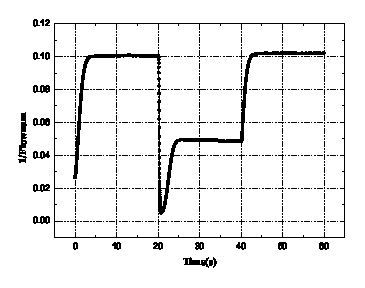
\includegraphics[width=2.5in]{flownum-pic-cut.eps}
\caption{The accuracy of estimation of flow number.}
\label{fig-flownum}
\end{figure}

\subsection{The performance of ECN Interest sending rate mechanism}

We use bottleneck topology to estimate the ECN Interest sending rate mechanism. The ECN Interest sending rate is calculated based on the principle that the bandwidth should be fully used. The ICP and ICP-shape use the TCP-style window control way. TCP-style window control way uses the timeout-principle to sense the congestion, and once timeout, it cut the interest window to half. TCP-style window control also use the slow-start to send the Interest. These will waste a lot of bandwidth. As Fig.~\ref{fig-linkuti} shows, ICP and ICP-shape waste bandwidth because of the slow start. The link utilization of ICP and ICP-shape is between 80\%-90\%. In contrast, even when the bottleneck link's bandwidth changes, the bandwidth utilization by smart-ECN always closes to 100\%.

\begin{figure}[t]
	\centering
	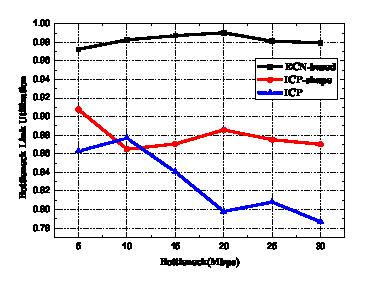
\includegraphics[width=2.5in]{utilization-pic-cut.eps}
	\caption{The bottleneck's link utilization compared with ICP and ICP-shape when change the bottleneck bandwidth.}
	\label{fig-linkuti}
\end{figure}

Because the ECN Interest sending rate makes sure that the rate can not exceed the bandwidth, almost no packets (no matter Interest or Data) drop in ECN interest sending rate mechanism, as the Fig.~\ref{fig-drop} shows. ICP uses timeout as the signal to inform congestion, and timeout is caused by dropping Data. In ICP, once the link become congested, the only solution is to drop Data, so the number of dropped Data is very large, as Fig.~\ref{fig-drop} shows. The ICP-shape shapes Interest before congestion happens, so it can reduce the number of Data needed to be dropped because of congestion. But as the delay of sending back and the difficulty of estimating the congestion, there are still some dropped Data.

\begin{figure}[t]
	\centering
	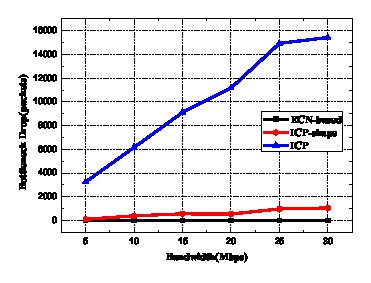
\includegraphics[width=2.5in]{drop-pic-cut.eps}
	\caption{The number of dropping packets in bottleneck compared with ICP and ICP-shape when change the bottleneck bandwidth.}
	\label{fig-drop}
\end{figure}

As Eq.~\ref{eq:updated_rt5} shows, the packets in the queue should do the utmost to be drained. This principle makes sure that in smart-ECN, the packets in the queue are always close to 0, as shown in Fig.~\ref{fig-queue}. In ICP, to use the bandwidth effectively, the receivers always try to enlarge the Interest window until the Data fills up the queue and the Data is dropped, so the packets in the queue is large. In ICP-shape, the router can shape Interest when it sense that congestion will happen. So in ICP-shape, the queue size is smaller than ICP, as shown in Fig.~\ref{fig-queue}.

\begin{figure}[t]
	\centering
	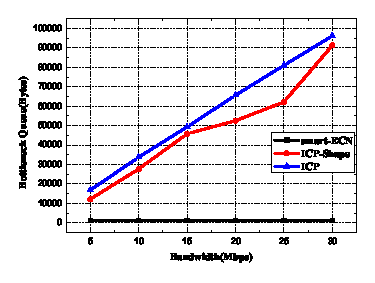
\includegraphics[width=2.5in]{queu-pic-cut.eps}
	\caption{The volume of queuing packets in bottleneck compared with ICP and ICP-shape when change the bottleneck bandwidth.}
	\label{fig-queue}
\end{figure}

Fig.~\ref{fig-fct} shows the FCT of different flows. Flow complete time in NDN is defined as the time from when receiver sends the first Interest until the receiver receives the last Data of the flow. The ECN Interest sending rate mechanism's link utilization is much higher than ICP. ECN Interest sending rate mechanism fairly applies bandwidth resource to all the flows, so even if the short flow can get fair bandwidth resource. No matter flows are short or long, their FCT are much better than ICP, as Fig.~\ref{fig-fct} shows.

\begin{figure}[t]
	\centering
	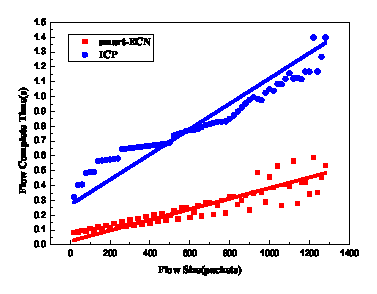
\includegraphics[width=2.5in]{fct-cut.eps}
	\caption{Smart-ECN's flow complete time compared with ICP.}
	\label{fig-fct}
\end{figure}

\subsection{Flow complete time compared with ICP}

We demonstrate the effectiveness of smart adaptive forwarding mechanism using mesh network topology. The total bottleneck bandwidth means the sum of bottleneck bandwidth on all the available paths. Using the forwarding-assistance and route information, the smart adaptive forwarding mechanism can choose a network-wide best path. The adaptive mechanism chooses the best forwarding interface just by the next hop's link information. As the next hop link information can not reflect the whole path's information, the adaptive mechanism will sometimes choose a wrong path whose later link is shared by far more flows. The non-adaptive mechanism chooses the path just by the route information, similar with TCP/IP. The non-adaptive mechanism can not change the forwarding interface according the network condition. As Fig.~\ref{fig-tfct} shows, under different total bandwidth, the smart adaptive forwarding's TFCT is much better than non-adaptive mechanism. As smart adaptive forwarding mechanism can choose a best path on the network-wide view, it's total flow complete time is even better than adaptive mechanism.

\begin{figure}[t]
	\centering
	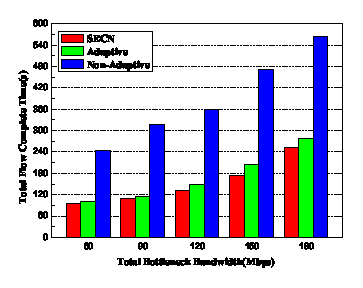
\includegraphics[width=2.5in]{adaptive-pic-cut.eps}
	\caption{Total flow complete time compared with other two forwarding mechanisms.}
	\label{fig-tfct}
\end{figure}


\section{Conclusion}
\label{sec:conclude}

We propose an ECN congestion control and smart forwarding mechanism in NDN. Data carries the ECN information to receivers. Receivers use ECN information to adjust its Interest sending rate. Under smart forwarding mechanism, routers choose the best forwarding interface using the SDN controller's network-view information. The ECN transport mechanism can ultimately use the link utilization and reduce the dropping packets. By joining the smart forwarding and ECN transport mechanism, the whole network resource can be effective used and total flow complete time can be reduced.

\begin{thebibliography}{1}

\bibitem{NDN}
V. Jacobson, D. K. Smetters, J. D. Thornton, M. F. Plass, N. H. Briggs,
and R. L. Braynard, ``Networking named content," in Proceedings of ACM
CoNEXT, 2009.
\bibitem{ICP}
G. Carofiglio, M. Gallo, and L. Muscariello, ``ICP: Design and evaluation
of an interest control protocol for content-centric networking," in Proc.
1st IEEE Int��l Workshop on Emerging Design Choices in Name-Oriented
Networking, 2012.
\bibitem{Adaptive}
C. Yi, A. Afanasyev, L. Wang, B. Zhang, and L. Zhang, ``Adaptivd forwarding
in named data networking," in SIGCOMM Comput.Commun.Rev, 2012.
\bibitem{CCTCP}
L. Saino, C. Cocora, and G. Pavlou, ``CCTCP: A scalable receiver-driven
congestion control protocol for content centric networking," in Proc.IEEE ICC Int��l Conference, 2013.
\bibitem{shape}
N. Rozhnova and S. Fdida, ``An effective hop-by-hop interest shaping
mechanism for ccn communications," in Proc.1st IEEE Int��l Workshop on Emerging Design Choices in Name-Oriented Networking, 2012.
\bibitem{SDN}
A. Voellmy and J. Wang, ``Scalable software defined network controllers," in ACM SIGCOMM Computer Communication Review, 2012
\bibitem{XCP}
D. Katabi, M. Handley and C. Rohrs, ``Congestion control for high
bandwidth-delay product networks," in Proc.of ACM SIGCOMM,2002.
\bibitem{RCP}
N. Dukkipati, M. Kobayashi, R. Zhang-Shen, and N. McKeown, ``Processor
sharing flows in the internet," in IWQOS, 2006.
\bibitem{TCP}
V. Jacobson, ``Congestion avoidance and control," in SIGCOMM Comput.Commun.Rev, 1988.
\bibitem{selfish}
L. Qiu, Y. R. Yang, Y. Zhang, and S. Shenker, ``On selfish routing in internet-like environments," in Proc. of the ACM SIGCOMM,2003.
\bibitem{ndnroute}
R. Ahmed, and M. F. Bari, `` $\alpha$Route: A Name Based Routing Scheme for Information Centric Networks," in Proc. of IEEE INFOCOM 2013.
\bibitem{NDNanalysis}
S. Braun, M. Monti, M. Sifalakis and C. Tschudin, ``An empirical study of
receiver-based AIMD flow control strategies for CCN," in IEEE ICCCN,2013.
\bibitem{Flow}
S. Oueslati, J. Roberts, and N. Sbihi, ``Flow-aware Traffic Control for
a  Content -Centric Network," in IEEE INFOCOM, 2012.
\bibitem{Multipath}
G. Carofiglio, M. Gallo, and L. Muscariello, ``Multipath congestion control in content-centric networks," in IEEE INFOCOM, 2013.
\bibitem{Contug}
S. Arianfar, P. Nikander, L. Eggert, and J. Ott, ``Contug: A receiver driven transport protocol for content-centric networks," in IEEE ICNP 2010 (Poster session),2010.
\bibitem{tcpdeadline}
C. Wilson, H. Ballani, T. Karagiannis , and A. Rowtron, ``Better never than late: meeting deadlines in datacenter networks," in Proc. of the ACM SIGCOMM 2011.
\bibitem{improveshape}
Y. G. Wang, N. Rozhnova, A. Narayanan, D. Oran, and I. Rhee, ``An improved hop-by-hop interest shaper for congestion control in named data networking," in Proc. Of ACM SIGCOMM ICN, 2013.
\bibitem{ndnsimnet}
http://ndnsim.net/
\bibitem{ndnsim}
A. Afanasyev, I. Moiseenko, and L. Zhang, ``ndnSIM: NDN simulator for NS-3," in NDN, Technical Report NDN-0005, 2012.


\end{thebibliography}


% that's all folks
\end{document}


